\section{The Neuron \& Activation Functions}
\begin{frame}{Meet the Neuron}
    \centering
    % \vspace{1em}
    
    \begin{tcolorbox}[colback=green!5, colframe=green!50!black, width=0.7\linewidth, arc=10pt]
        \centering
        \Large
        \textbf{The magic building block is called a Neuron.}
    \end{tcolorbox}
    
    \vspace{2em}
    
    \begin{columns}[c]
        \begin{column}{0.45\textwidth}
            \centering
            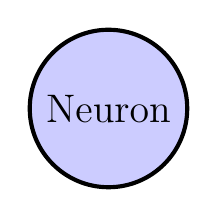
\begin{tikzpicture}[scale=1.2]
                \node[circle, draw, fill=blue!20, minimum size=2cm, line width=1.5pt] (n) {\Large Neuron};
            \end{tikzpicture}
        \end{column}
        
        \begin{column}{0.1\textwidth}
            \centering \Huge $\to$
        \end{column}
        
        \begin{column}{0.45\textwidth}
            \centering
            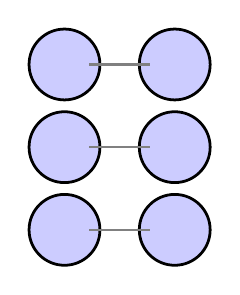
\begin{tikzpicture}[scale=0.7]
                % Stack of Neurons
                \foreach \x in {0, 2} 
                    \foreach \y in {0, 1.5, 3} 
                        \node[circle, draw, fill=blue!20, minimum size=0.9cm, line width=1pt] at (\x, \y) {};
                
                % Connections
                \draw[gray, thick] (0.45, 3) -- (1.55, 3);
                \draw[gray, thick] (0.45, 1.5) -- (1.55, 1.5);
                \draw[gray, thick] (0.45, 0) -- (1.55, 0);
            \end{tikzpicture}
        \end{column}
    \end{columns}
    
    \vspace{1.5em}
    \pause
    \textit{But how powerful can these simple blocks really be?}
\end{frame}


% --- SLIDE 4: The Theory ---
\begin{frame}{Surprisingly Powerful: Universal Approximation}
    \begin{columns}[c]
        \begin{column}{0.5\textwidth}
            Here's the remarkable part: if you stack enough neurons together, they can learn to fit \textbf{any pattern}, no matter how simple/complex it is.
            
            \vspace{1em}
            \begin{tcolorbox}[colback=yellow!10, colframe=orange!60, title=\textbf{Universal Approximation Theorem}]
                \small
                A Neural Network with enough neurons can approximate \textbf{any continuous function} to arbitrary accuracy.
            \end{tcolorbox}

            \vspace{0.5em}
            \small This is why neural networks are so flexible and powerful!
        \end{column}
        
        \begin{column}{0.50\textwidth}
            \centering
            
            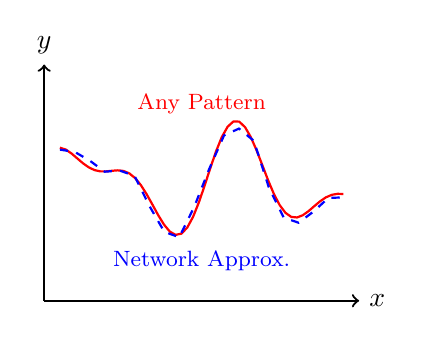
\begin{tikzpicture}[scale=1.0]
                \draw[->, thick] (0,0) -- (4,0) node[right] {$x$};
                \draw[->, thick] (0,0) -- (0,3) node[above] {$y$};
                
                % Complex Function
                \draw[red, thick, domain=0.2:3.8, samples=50] plot (\x, {1.5 + 0.5*sin(\x*180) + 0.3*cos(\x*300)});
                \node[red, font=\footnotesize] at (2, 2.5) {Any Pattern};
                
                % Approximation
                \draw[blue, thick, dashed, domain=0.2:3.8, samples=20] plot (\x, {1.5 + 0.5*sin(\x*180) + 0.3*cos(\x*300) + 0.1*rand});
                \node[blue, font=\footnotesize] at (2, 0.5) {Network Approx.};
            \end{tikzpicture}
            
            \vspace{0.5em}
            \small \textit{"Give me enough neurons, \\and I can fit any function."}
        \end{column}
    \end{columns}

    \pause
    \vspace{1em}
    \centering
    \textit{So let's look inside: what does a neural network actually look like?}
\end{frame}

% =========================
% 2. Anatomy of a Neural Network
% =========================
\section{Anatomy of a Neural Network}

% --- SLIDE 5: The Architecture ---
\begin{frame}{Inside a Neural Network}
    \begin{columns}[c]
        \begin{column}{0.55\textwidth}
            A Neural Network is organized into \textbf{layers} of neurons, where each layer transforms the data step by step.
            
            \vspace{1em}
            \textbf{The Three Parts:}
            \begin{itemize}
                \item \textbf{Input Layer:} Receives your raw data ($x$).
                \item \textbf{Hidden Layers:} Extract patterns and features.
                \item \textbf{Output Layer:} Produces the final prediction ($\hat{y}$).
            \end{itemize}
            
            \vspace{0.8em}
            \small The "deep" in Deep Learning comes from having many hidden layers.
        \end{column}
        
        \begin{column}{0.45\textwidth}
            \centering
            % Simple Network Diagram
            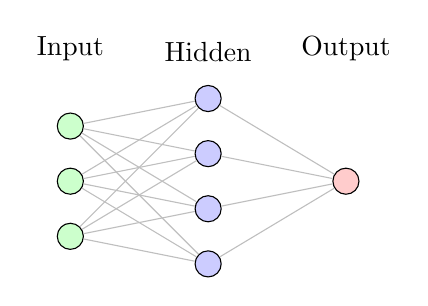
\begin{tikzpicture}[scale=0.7]
                % Draw nodes
                \foreach \i in {1,2,3} \node[circle,draw,fill=green!20] (I\i) at (0,-\i) {};
                \foreach \i in {1,2,3,4} \node[circle,draw,fill=blue!20] (H\i) at (2.5,-\i+0.5) {};
                \node[circle,draw,fill=red!20] (O) at (5,-2) {};
                
                % Draw edges
                \foreach \i in {1,2,3} \foreach \j in {1,2,3,4} \draw[gray!50] (I\i) -- (H\j);
                \foreach \j in {1,2,3,4} \draw[gray!50] (H\j) -- (O);
                
                % Labels
                \node[above] at (0,0) {Input};
                \node[above] at (2.5,0) {Hidden};
                \node[above] at (5,0) {Output};
            \end{tikzpicture}
            
            \vspace{1em}
            \small \textit{Each circle is a neuron,\\each line is a connection.}
        \end{column}
    \end{columns}

\end{frame}

\begin{frame}{Example: Predict House Price}
    \begin{figure}
        \centering
        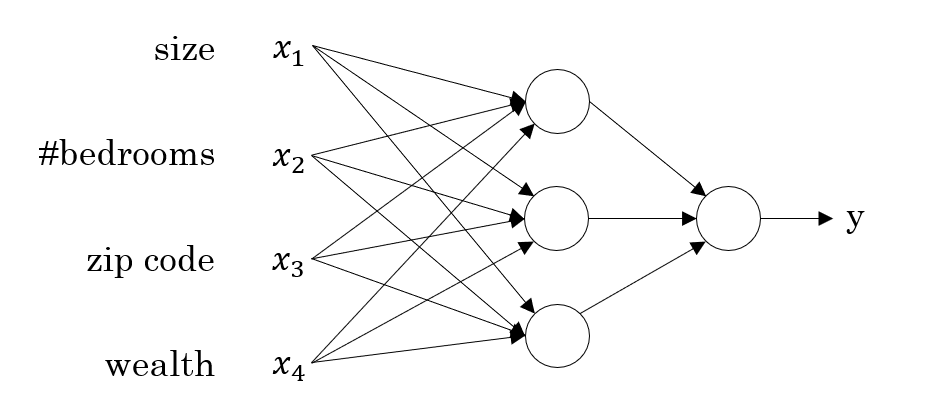
\includegraphics[width=\textwidth,height=0.7\textheight,keepaspectratio]{images/simple_neural_network.png}
    \end{figure}
\end{frame}


% --- SLIDE 5: The Architecture ---
\begin{frame}{Inside a Neural Network}
    \begin{columns}[c]
        \begin{column}{0.55\textwidth}
            A Neural Network is organized into \textbf{layers} of neurons, where each layer transforms the data step by step.
            
            \vspace{1em}
            \textbf{The Three Parts:}
            \begin{itemize}
                \item \textbf{Input Layer:} Receives your raw data ($x$).
                \item \textbf{Hidden Layers:} Extract patterns and features.
                \item \textbf{Output Layer:} Produces the final prediction ($\hat{y}$).
            \end{itemize}
            
            \vspace{0.8em}
            \small The "deep" in Deep Learning comes from having many hidden layers.
        \end{column}
        
        \begin{column}{0.45\textwidth}
            \centering
            % Simple Network Diagram
            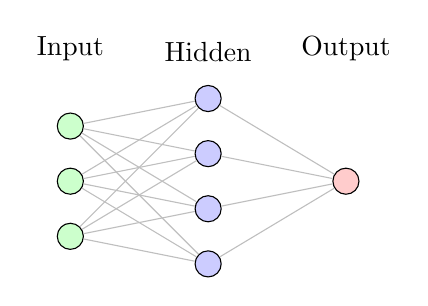
\begin{tikzpicture}[scale=0.7]
                % Draw nodes
                \foreach \i in {1,2,3} \node[circle,draw,fill=green!20] (I\i) at (0,-\i) {};
                \foreach \i in {1,2,3,4} \node[circle,draw,fill=blue!20] (H\i) at (2.5,-\i+0.5) {};
                \node[circle,draw,fill=red!20] (O) at (5,-2) {};
                
                % Draw edges
                \foreach \i in {1,2,3} \foreach \j in {1,2,3,4} \draw[gray!50] (I\i) -- (H\j);
                \foreach \j in {1,2,3,4} \draw[gray!50] (H\j) -- (O);
                
                % Labels
                \node[above] at (0,0) {Input};
                \node[above] at (2.5,0) {Hidden};
                \node[above] at (5,0) {Output};
            \end{tikzpicture}
            
            \vspace{1em}
            \small \textit{Each circle is a neuron,\\each line is a connection.}
        \end{column}
    \end{columns}
    
    \vspace{1em}
    \centering
    \textit{Now let's zoom in and see what a single neuron actually does...}
\end{frame}


% =========================
% 3. The Neuron: Building Block of Deep Learning
% =========================


% --- SLIDE 6: Single Neuron Computation ---
\begin{frame}{What Does a Neuron Do?}
    \begin{columns}[c]
        \begin{column}{0.45\textwidth}
            A neuron performs two simple operations:
            
            \vspace{1em}
            \textbf{1. Linear Combination:}
            \[
                z = w^\top x + b
            \]
            \small (Just like linear regression!)
            
            \vspace{1em}
            \textbf{2. Non-linear Activation:}
            \[
                a = \sigma(z)
            \]
            \small (This is the new part)
            
            \vspace{1em}
            \normalsize
            The output $a$ becomes the input for the next layer neurons!
        \end{column}
        
        \begin{column}{0.6\textwidth}
            % \centering
            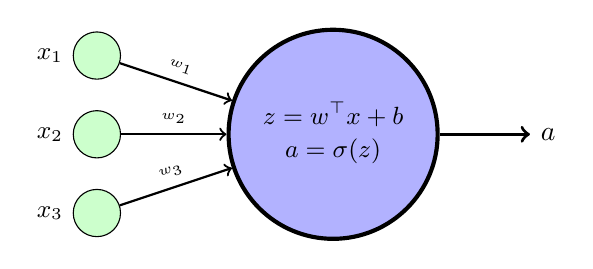
\begin{tikzpicture}[scale=1.0]
                % Input nodes
                \foreach \i in {1,2,3} {
                    \node[circle, draw, fill=green!20, minimum size=0.6cm] (x\i) at (0, -\i) {};
                    \node[left] at (x\i.west) {\small $x_{\i}$};
                }
                
                % Neuron
                \node[circle, draw, fill=blue!30, minimum size=1.8cm, line width=1.5pt] (neuron) at (3, -2) {
                    \begin{tabular}{c}
                        \small $z = w^\top x + b$ \\
                        \small $a = \sigma(z)$
                    \end{tabular}
                };
                
                % Connections with weights
                \foreach \i in {1,2,3} {
                    \draw[->, thick] (x\i) -- (neuron) node[midway, above, sloped] {\tiny $w_{\i}$};
                }
                
                % Output
                \draw[->, very thick] (neuron) -- (5.5, -2) node[right] {$a$};
            \end{tikzpicture}
        \end{column}
    \end{columns}
    
    \pause
    \vspace{0.8em}
    \centering
    \textit{But why do we need that activation function $\sigma$? Why don't we just use the linear part ($wx+b$)?}
\end{frame}

% --- SLIDE 7: Why Activations (SIMPLIFIED) ---
\begin{frame}{Why We Need Activation Functions}
    \textbf{Question:} Why don't we just use the linear part ($wx+b$)?
    
    \vspace{1em}
    \begin{alertblock}{The Problem: Linearity}
        Without activations, stacking linear layers gives us... just another linear function!
        $$ \text{Linear} + \text{Linear} = \text{Linear} $$
        No matter how many layers you stack, without activations, the whole network collapses into a single Linear Regression model!
    \end{alertblock}
    
    \pause
    \vspace{1em}
    \begin{tcolorbox}[colback=green!5, colframe=green!50]
        \textbf{Solution: The "Bend"}:
        Activations ($\sigma$) introduce non-linearity. 
        Think of it like bending a ruler. This allows us to fit curved, complex patterns.
    \end{tcolorbox}
\end{frame}

% % --- SLIDE 7: Why Activations ---
% \begin{frame}{Why We Need Activation Functions}
%     \textbf{The Problem:} Without activations, stacking layers gives us... just another linear function!
    
%     \vspace{1em}
%     \begin{tcolorbox}[colback=red!5, colframe=red!50]
%         \centering
%         \textbf{Without activations:}
%         \[
%             \text{Layer 1: } z_1 = W^{(1)} x + b^{(1)}
%         \]
%         \[
%             \text{Layer 2: } z_2 = W^{(2)} z_1 + b^{(2)} = W^{(2)}(W^{(1)} x + b^{(1)}) + b^{(2)}
%         \]
%         This is just $W_{\text{combined}} x + b_{\text{combined}}$ $\rightarrow$ still linear!
%     \end{tcolorbox}
    
%     \pause
%     \vspace{1em}
%     \begin{tcolorbox}[colback=green!5, colframe=green!50]
%         \centering
%         \textbf{Solution: Non-linear activations}
        
%         They introduce "bends" and "thresholds" that let the network approximate complex, non-linear patterns.
%     \end{tcolorbox}
    
%     % \vspace{0.8em}
%     \centering
%     \textit{What activation functions do we use?}
% \end{frame}

% --- SLIDE 8: Common Activations ---
\begin{frame}{Common Activation Functions}
    \vspace{6mm}
    \begin{columns}[T]
    
        \begin{column}{0.32\textwidth}
            \centering
            \textbf{ReLU}
            \[
                \sigma(z) = \max(0, z)
            \]
            
            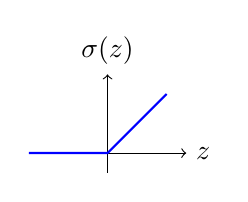
\begin{tikzpicture}[scale=0.5]
                \draw[->] (-2,0) -- (2,0) node[right] {$z$};
                \draw[->] (0,-0.5) -- (0,2) node[above] {$\sigma(z)$};
                \draw[thick, blue] (-2,0) -- (0,0) -- (1.5,1.5);
            \end{tikzpicture}
            
            \small
            \textbf{Most popular!} Simple and works well in deep networks.
        \end{column}
        
        \begin{column}{0.32\textwidth}
            \centering
            \textbf{Sigmoid}
            \[
                \sigma(z) = \frac{1}{1 + e^{-z}}
            \]
            
            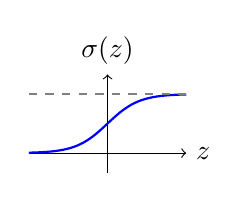
\begin{tikzpicture}[scale=0.5]
                \draw[->] (-2,0) -- (2,0) node[right] {$z$};
                \draw[->] (0,-0.5) -- (0,2) node[above] {$\sigma(z)$};
                \draw[thick, blue, domain=-2:2, samples=50] plot (\x, {1.5/(1+exp(-2.5*\x))});
                \draw[dashed, gray] (-2,1.5) -- (2,1.5);
            \end{tikzpicture}
            
            \small
            Output in $(0, 1)$. You know this from logistic regression!
        \end{column}
        
        \begin{column}{0.32\textwidth}
            \centering
            \textbf{Tanh}
            \[
                \sigma(z) = \tanh(z)
            \]
            
            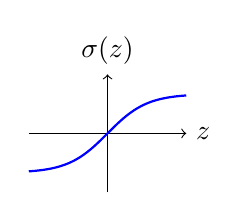
\begin{tikzpicture}[scale=0.5]
                \draw[->] (-2,0) -- (2,0) node[right] {$z$};
                \draw[->] (0,-1.5) -- (0,1.5) node[above] {$\sigma(z)$};
                \draw[thick, blue, domain=-2:2, samples=50] plot (\x, {tanh(\x)});
            \end{tikzpicture}
            
            \small
            Output in $(-1, 1)$. Similar to sigmoid but centered at zero.
        \end{column}
    \end{columns}
\end{frame}

% --- SLIDE: From Neurons to Layers (The Missing Link) ---
% --- SLIDE 9A: Scaling Up (Concept) ---
